%-----------------------------------------------------------------
% Tomas James
% 3rd Year Project: Exoplanet Detection and Characterisation
% Cardiff University
%-----------------------------------------------------------------

%-----------------------------------------------------------------
% Start Document Preamble
%-----------------------------------------------------------------

\documentclass{article}

\usepackage{amsmath} % Maths typesetting
\usepackage{fancyhdr}

\usepackage[english]{babel}% Recommended
\usepackage{csquotes}% Recommended

\usepackage[style=authoryear-ibid, backend=biber]{biblatex}

% \bibliography{<mybibfile>}% ONLY selects .bib file; syntax for version <= 1.1b
\addbibresource{/Users/tomasjames/Documents/University/Cardiff/Project/Project/Reports/Interim/Master/tex/test.bib}% Syntax for version >= 1.2

\pagestyle{fancy}
\fancyhf{}

\usepackage{graphicx}

% Define title and author
\title{Exoplanet Characterising and Observation}
\author{\textsc{Tomas James}}

%-----------------------------------------------------------------
% Begin Document
%-----------------------------------------------------------------

\begin{document}

% Insert date
\date{\today}

%\pagerange{\pageref{firstpage}--\pageref{lastpage}} \pubyear{2014}

\maketitle

\label{firstpage}

%-----------------------------------------------------------------
% Begin Abstract
%-----------------------------------------------------------------

\begin{abstract}
For this project, the transiting extrasolar planets WASP-22 b, WASP-78 b and HATS-5 b were chosen to be observed using LCOGT telescopes in the Southern Hemisphere. The data obtained from these observations will then be used to computationally model the observed transit, allowing the calculation of orbital and physical parameters about each exoplanet. Conclusions about each planet will be compared and contrasted to the other planets observed. The parameters determined will also be compared to the known quantities for each planet.
\end{abstract}

%-----------------------------------------------------------------
% Introduction
%-----------------------------------------------------------------

\section{Introduction}
The discovery of the first extrasolar planet by \textcite{first} introduced a developing field into astronomical research that is now one of the most exciting and fast moving fields in modern astrophysics. Subsequent detections, such as the first main-sequence extrasolar planet by \textcite{MQ} continue to reveal a more diverse and rich spectrum of exoplanets. More than 20 years on from these detections, the \textcite{exo} records 1853 \footnote{As of Monday 8th December 2014} extrasolar planets that have been discovered using a variety of detection methods utilising both ground and satellite based telescopes in a multitude of collaborative missions. These vary from discovering new exoplanets to actively searching for Earth analogs that could, under the right circumstances, harbor life.

\subsection{Extrasolar Planets}
Extrasolar planets - or exoplanets - are planetary objects orbiting stars outside of the Solar System.  

In the early 21st century, space telescopes such as Kepler and CoRoT were launched in order to begin detecting and characterising exoplanets. Uniquely these missions could observe a wide distribution of exoplanets, effectively allowing the formation and evolution of planetary systems to be observed. Ground based telescopes such as KELT and the CORALIE Spectrograph continue to operate but are prone to atmospheric effects, limiting their effectiveness in comparison to space based telescopes.

\subsection{Detection Methods}
Extrasolar planet detection methods are divided into two classes: direct and indirect detections. A direct detection uses data that explicitly shows the presence of an extrasolar planet. An indirect detection uses effects that an extrasolar planet has on its parent star to infer the planet's existence. To date there are 5 well established detection methods. These are discussed below.



\subsubsection{Transiting}
When an object that does not produce its own light, such as an exoplanet, passes across the line of sight between the observer and a very luminous object, such as a star, a dip in the total luminosity of the system is observed owing to the exoplanet blocking a portion of the star's flux from the observer. By plotting the total flux received as a function of time the presence of an exoplanet can be suggested if a dip in the total flux received is observed. An example of a lightcurve can be seen in Figure ~\ref{Transit}.

\begin{figure}
\centering
    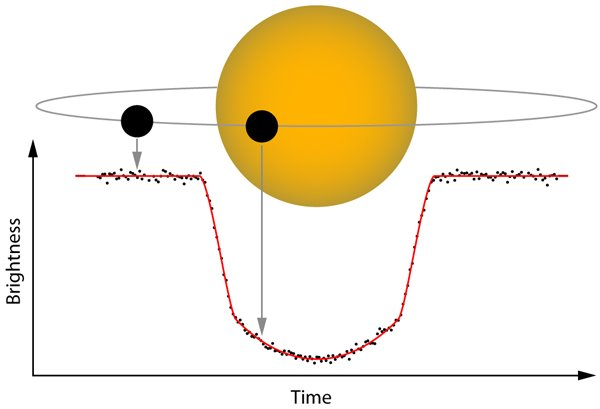
\includegraphics[scale = 0.5]{/Users/tomasjames/Documents/University/Cardiff/Project/Project/Reports/Interim/Master/img/Saved/transit}
\caption[An example showing how the presence of an exoplanet moving across a star results in a reduction in the observed flux, as evidenced by the visible ingress.]{An example showing how the presence of an exoplanet moving across a star results in a reduction in the observed flux, as evidenced by the visible ingress \parencite{transitimg}}.\label{Transit}
\end{figure}

This method has various limitations however. For example, bias exists towards exoplanets with large radii and small orbital periods as they block more of the star’s flux incident upon the observer more often, allowing more reliable estimates of parameters like exoplanetary radius to be determined. Another limitation is that exoplanets with orbital inclinations of 90$^\circ$ cannot be detected as they do not pass in front of their host star relative to the observer.

Moreover, any partially opaque object passing infront of a star will have the effect of blocking a portion of the star's total flux. \textcite{false} estimated that this is a rare occurence, with the false positive probability (FPP)\footnote{The FPP is the probability that the exoplanet detected is a false positive, or an astronomical object passing between the telescope and the star, therefore acting as an erroneous detection.} being estimated at $<10\%$ for almost 90\% of candidates being observed by the Kepler mission.

\subsubsection{Radial Velocity
}
The existence of an exoplanetary companion orbiting a host star alters the system's centre of mass causing both the exoplanet and host star to orbit about it. As a direct result of this the radial velocity of the star changes over time, peaking at a maximum when the star is moving directly toward, or away from, the observer. Conversely the radial velocity of the star is at a minimum when the star moves normal to the observer’s line of sight. This is demonstrated in Figure~\ref{rvdetect}.

\begin{figure}
\centering
    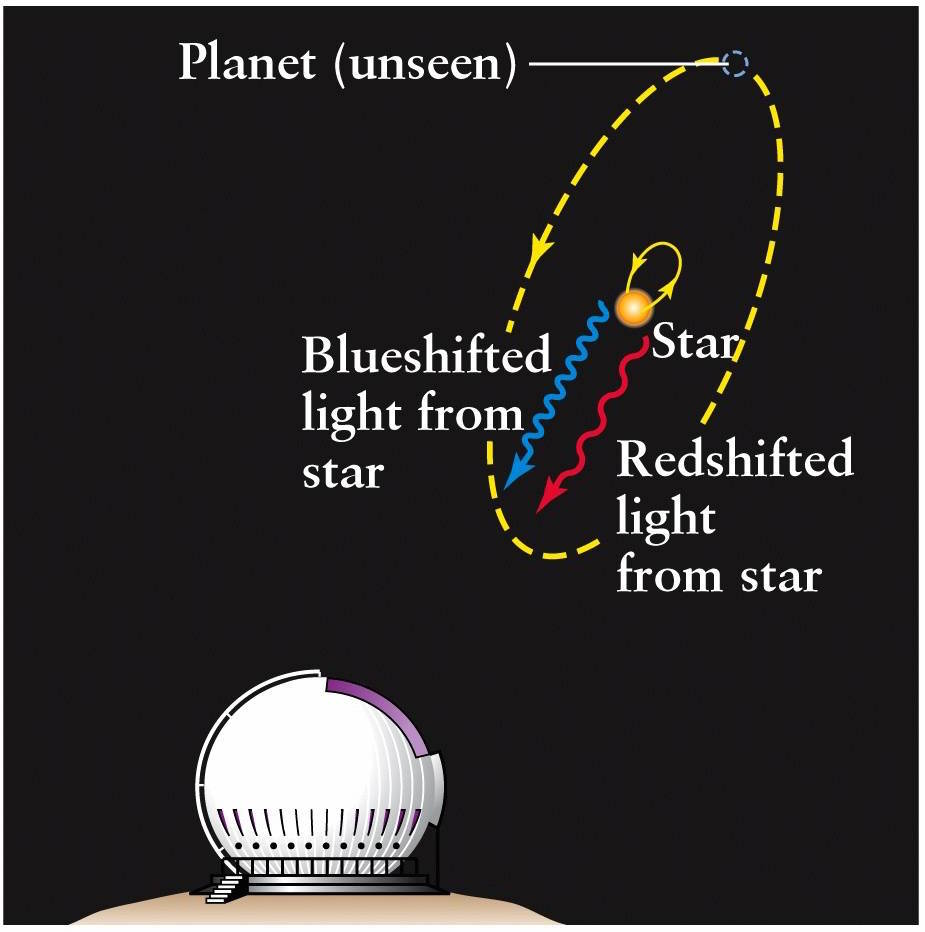
\includegraphics[scale = 0.2]{/Users/tomasjames/Documents/University/Cardiff/Project/Project/Reports/Interim/Master/img/Saved/radialvelocity}
\caption[An example showing how the presence of a hidden exoplanet induces a change in the centre of mass of the planetary system, therefore altering the centre of orbit of each of the system's orbiting companions. This can be detected by the resulting Doppler shift of the host star's spectral lines.] {An example showing how the presence of a hidden exoplanet induces a change in the centre of mass of the planetary system, therefore altering the centre of orbit of each of the system's orbiting companions. This can be detected by the resulting Doppler shift of the host star's spectral lines \parencite{rvdetect}}.\label{rvdetect}
\end{figure}

This variation is detected by observing the Doppler shift of the star’s spectral lines. Whilst the star is moving towards the observer a decrease in the wavelength of the spectral lines is observed. When it is moving away from the observer an in the wavelength of the spectral lines is observed. No change is observed when the star is moving normal to the observer’s line of sight.


This detection method is heavily biased towards large exoplanets orbiting less massive stars with small orbital periods, owing to the larger perturbation observed in the host star’s orbit, which in turn increases the probability of detection. A common source of error using the radial velocity method relates to the expansion and contraction of the star itself. This produces a very similar spectroscopic signature that would be expected to be observed were the star's orbit to be perturbed by an exoplanet.

\subsubsection{Direct Imaging
}
Direct imaging detections utilise the thermal emission of an extrasolar planet to detect the planet as a source of infrared radiation in an image taken in the infrared. 

The method of direct imaging is heavily biased towards large, hot planets that are seperated by a large distance from their host star. This highlights a major disadvantage that direct imaging has: exoplanets lying close to a large, luminous star will be hidden owing to the large infrared luminosity difference between the two objects.

 

Typically this limitation is solved by the attachment of a coronograph which blanks out the host star to avoid complications relating to its presence in the image. This is especially useful for solving problems related to the large infrared luminosity difference between a star and planet. It also allows for adjustments in exposure time, as the highly luminous star would no longer dictate the maximum exposure, therefore allowing longer exposure times leading to the potential discovery of cool exoplanets. 

\subsubsection{Microlensing
}
Microlensing detections use the principle of gravitational microlensing to infer the presence of an exoplanet. The light from a luminous object behind the star in the observer's line of sight is lensed as it encounters the strong gravitational field of the exoplanetary system. Any irregularities in the known distortion caused by the lensing suggests the presense of an orbiting exoplanet.  

For microlensing detections to be possible a luminous object must exist beyond the line of sight between the observer and the exoplanetary system.

\subsubsection{Pulsar Timing}
Pulsar timing detections rely on the regular, periodic bursts of radio emission from an ultradense, rapdily rotating neutron star - a pulsar. 

Traditionally this radio emission - owing to its stability and reliability - has been used to track the orbital period of the star, but if a planetary companion is orbiting the pulsar then small orbital perturbations are to be expected owing to the orbit of the system about a common centre of mass. This results in periodic anomalies in the detection of the emitted radio signal as the star moves around the centre of mass of the system. Tracking these anomalies allows the period of the star to be determined and crucially, the mass and orbital parameters of the exoplanet as well.

Pulsar timing was used by \autocite{first} to detect the first exoplanet orbiting the pulsar PSR1257+12 in 1992. 

The reliability and accuracy of the pulsar timing method allows much smaller exoplanets to be detected. According to the \textcite{exo} only 16 exoplanets have been detected using this method since 1992, indicating that exoplanets orbiting pulsars are rare.

%-----------------------------------------------------------------
% Pre Data Collection Tests
%-----------------------------------------------------------------

\subsection{Reviewing the Mechanics of Exoplanetary Orbits}
To better understand the exoplanetary properties and their orbital behaviour the \textcite{exo} was used to download\footnote{The last download of this data was 17\textsuperscript{th} October 2014} data on all detected exoplanets. A Python script was written to process this data with the primary aim of reducing it to graphs that could reveal trends between the quantities plotted.

\begin{figure}
\centering
    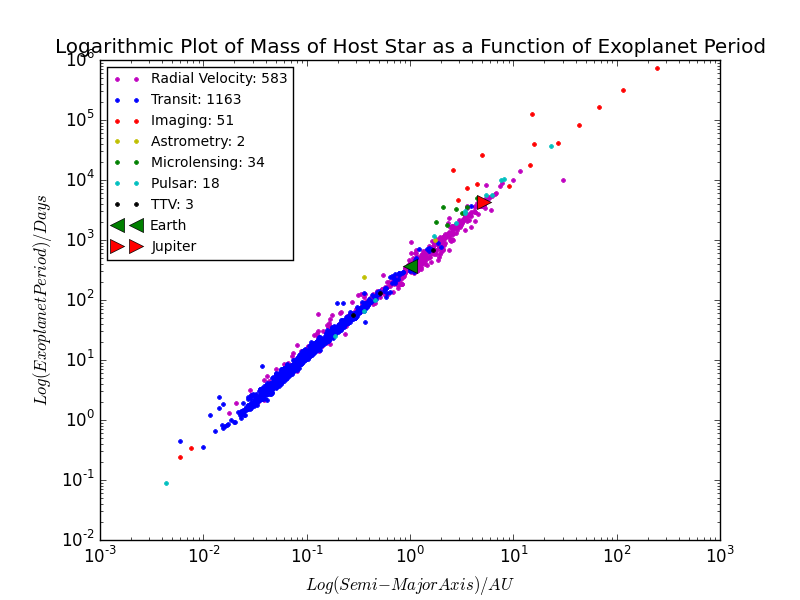
\includegraphics[scale = 0.4]{/Users/tomasjames/Documents/University/Cardiff/Project/Project/Reports/Interim/Master/img/log_period_major}
\caption{A loglog plot showing the relationship between an exoplanet's period and its semi-major axis.}\label{log_period_major}
\end{figure}

\subsection*{Figure~\ref{log_period_major}}
As can be seen in figure~\ref{log_period_major} the loglog plot of orbital period vs semi-major axis produces a very well defined and characteristic straight line. Kepler's 3rd Law relates period and semi-major axis as defined in equation \ref{Kepler}.

\begin{equation} \label{Kepler}
    T^{2} \propto a^{3} 
\end{equation}

In this instance T is the orbital period and a is the semi-major axis. Given that orbital systems are bound by Kepler's Laws (the Jupiter and Earth points confirm that this is the case for those 2 Solar System planets) the shape of the graph is to be expected. Interestingly a number of points lie off the main sequence of data in figure ~\ref{log_period_major}. Regrettably the \autocite{exo} does not include error estimations for all exoplanet entries, meaning firm conclusions about why these points lie off of the main sequence cannot be drawn without speculation. 

Figure ~\ref{log_period_major} also allows analysis of the sensitivity of each detection method. For example the exoplanet with the fastest orbital period and smallest semi-major axis was detected using the pulsar timing method, whilst the exoplanet with the slowest period and largest semi-major axis was detected using the direct imaging method. Direct imaging does however detect exoplanets across the most diverse range of periods and semi-major axes of those detection methods considered, ranging from the second-smallest semi-major axis to the largest. 

\begin{figure}
\centering
    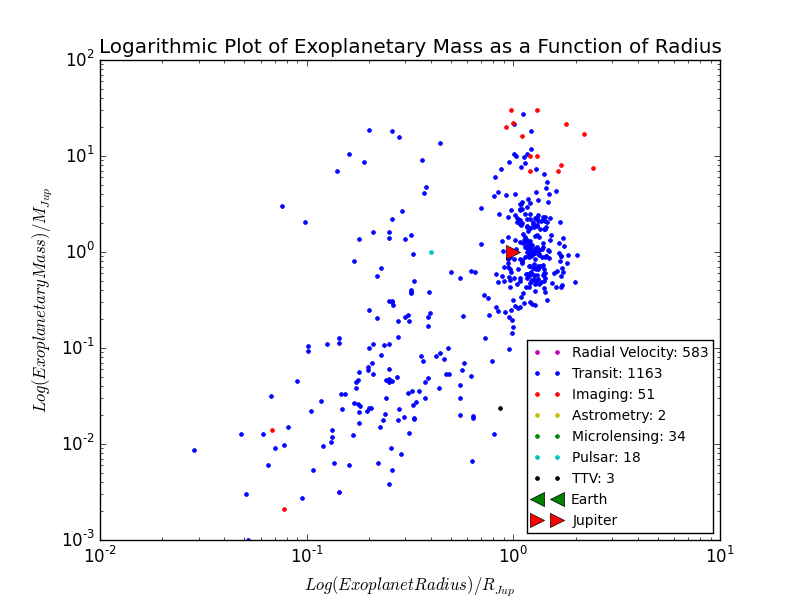
\includegraphics[scale = 0.4]{/Users/tomasjames/Documents/University/Cardiff/Project/Project/Reports/Interim/Master/img/log_radius_mass}
\caption{A loglog plot showing the relationship between an exoplanet's mass and its radius.}\label{log_radius_mass}
\end{figure}

\subsection*{Figure~\ref{log_radius_mass}}
Considering Figure~\ref{log_radius_mass}, less of an observed trend is immediately visible when compared to Figure~\ref{log_period_major}. The data does, however, exhibit an increasing trend towards larger mass and radii.  

Mass and radius are linked through equation~\ref{density}. 

\begin{equation} \label{density}
    m = \frac{4}{3}\pi R^3 \rho
\end{equation}

 where $m$ is the planetary mass, $R$ is the planetary radius and $\rho$ is the planetary density. If equation~\ref{density} describes the profile shown in Figure~\ref{log_radius_mass}, then the deviation from constant positive correlation is due to $\rho$ varying (i.e. $\rho$ is not constant across all exoplanets). 

 Interestingly a grouping of data points exists close the 1 $R_Jup$ marker, indicating a large number of exoplanets having a radius close to this value. The cause of this isn't immediately apparent, so further investigation is required to determine why this grouping exists.

 Figure~\ref{log_radius_mass} also highlights how dominant the transit detection method is, having twice the number of confirmed detections than all other detection methods combined. It also confirms that the transit method can detect exoplanets across the largest mass range. Both Figures~\ref{log_period_major} and ~\ref{log_radius_mass} follow confirmed mathematical trends and show that the Solar System isn't an anomolous planetary system. 

%-----------------------------------------------------------------
% Observatory Information 
%-----------------------------------------------------------------

\subsection{LCOGT Observatories}
Observations were limited to LCOGT sites in the Southern Hemisphere owing to a greater number of available telescopes lying south of the equator. These sites are listed in table ~\ref{observatory}.

\begin{table}
    \centering
    \begin{tabular}{ | l | l | l | }
    \hline \hline
    Observatory & Latitude (Deg) & Longitude (Deg)       \\ \hline \hline
    Cerro Tololo    & 30$^\circ$ 10' 2.64"S & 70$^\circ$ 48' 17.28"W  \\
    Sutherland   & 32$^\circ$ 22' 48"S & 20$^\circ$ 48' 36"E  \\
    Siding Spring  & 31$^\circ$ 16' 23.88"S & 149$^\circ$ 4' 15.6"E \\
    \hline
    \end{tabular}
    \caption{A table showing the observatories housing LCOGT telescopes that were used for data collection during this project \parencite{sites}.}
    \label{observatory}
\end{table}

As all of the sites in table ~\ref{observatory} house 1.0m Ritchey-Chretien Cassegrain telescopes, it was this variety of instrument that was used to collect data. Of all of these sites however, Siding Spring is the only telescope to currently have both a 2.0m and 1.0m Ritchey-Chretien variant. 

Each 1.0m telescope allows for the selection of 2 different sensors, along with a range of filters \parencite{1m}.

\begin{itemize}

  \item SBIG STX-16803, FOV 16x16 arcmin
  \item Sinistro Fairchild CCD-486 BI, FOV 27x27 arcmin

\end{itemize} 

This project focused on using the SBIG sensor for each observed transit as it was this sensor that was installed at all sites at the time of observations. [The .FITS header shows the SBIG sensor was used for observations at CT - is this incorrect?]

Each of the candidates considered had peak brightnesses in the UV band, therefore meaning that the Bessell-I filter - with wavelength centre at 798 nm over a width of 154 nm - was the primary choice. This was chosen in order to ensure that the brightness difference between the host star and exoplanet was great enough to produce a large and visible ingress.

%-----------------------------------------------------------------
% Exoplanets for Consideration
%-----------------------------------------------------------------

\section{Exoplanets for Observation}
Observations were required to be obtained during the time frame October 2014 - December 2014. To determine which exoplanets were visible during this period, the STARALT tool \parencite{staralt} was used in conjuction with the Exoplanet Transit Database \parencite{etd}. Only transiting exoplanets were considered for this project as equipment required for other detection methods was not available at the observatories used. 

Once the number of visible sources was determined, the number of those sources that were undergoing visible transits during the required time period was determined using the ETD's Transit Prediction function. These were crossreferenced using the STARALT function STARMULT, which produces an optimal observing date for a given source based on the observatory coordinates in table \ref{observatory} and stipulation that observations must occur above an altitude of 30$^\circ$\footnote{The airmass below this altitude would have rendered any observations highly prone to errors from atmospheric effects} above the horizon. The candidates for observation can be seen in Table ~\ref{planets}.

\begin{table}
    \centering
    \begin{tabular}{ | l | l | l | l | }
    \hline \hline
    Exoplanet & RA & Dec & Date       \\ \hline \hline
    WASP-22 b    & 03h 31m 16.3s & -23$^\circ$ 49' 11" & 09/11/2014 \\
    WASP-78 b   & 04h 15m 02.0s & -22$^\circ$ 06' 59.1" & 30/11/2014 \\
    HATS-5 b  & 04h 28m 53.47s & -21$^\circ$ 28' 54.0" & 01/12/2014 \\
    \hline
    \end{tabular}
    \caption{A table showing the exoplanets to be observed in this project along with the proposed date of observation and the coordinates, in RA/Dec, of each source \parencite{etd}.}
    \label{planets}
\end{table}

%-----------------------------------------------------------------
% Methodology
%-----------------------------------------------------------------

\section{Methodology}
\subsection{Data Collection}
In order to determine the best exposure times for each candidate, initial test exposures
were assigned to each system - these test exposures varied in 10s integration time
increments from 30s - 90s. The resulting files were then assessed manually to determine
the quality of the data and subsequently the best integration time.

This process determined that 90s exposures for all systems generated the best quality
data. A longer exposure time is preferable in order to maximise the SNR\footnote{$SNR 
\propto \sqrt{t}$ where t is the integration time}. 

For an exoplanet to be characterised it is necessary to observe the system as many times as possible over the duration of the transit. A baseline flux outside of the transit is also needed in order for the transit itself to be visible, so exposures were started 15 minutes before the estimated transit start (i.e. 15 minutes before the planet first occults the host star) and concluded 15 minutes after the transit ended. The optimum number of exposures was calculated using equation \ref{exposure}. 

\begin{equation} \label{exposure}
    N_{e} = \frac{D_{transit} + 2t_{window}}{t_{e} + t_{read}}
\end{equation}

In equation \ref{exposure}, $N_{e}$ is the maximum number of exposures, $D_{transit}$ is the transit duration in seconds, $t_{window}$ is the time between observations beginning and transit beginning, $t_{e}$ is the exposure time in seconds and $t_{read}$ is the necessary readout time for the telescope in use. In this case, $t_{window}=900s$ and $t_{read}=15s$.

Whilst $N_{e}$ is the theoretical maximum number of exposures possible, this was reduced by a relative number of exposures to allow the telescope in use to prepare for the next exposure in ample time. 

LCOGT's online scheduler was used to insert the observation requests into the observation queue.

\subsection{Data Analysis}
LCOGT systems use data reduction pipelines based upon the ORAC-DR infrastructure developed by \textcite{orac-dr} for UKIRT and JCMT initiatives. The pipeline reducing data from the LCOGT system runs multiple independent recipes for bad-pixel masking, bias subtraction, flat field correction and WCS fitting \parencite{pipeline}.  

The resulting pipeline reduced and corrected data was then downloaded from the LCOGT Data Archive and analysed. In the case of this project the primary form of data analysis comprised of aperture photometry using the GAIA package, available as part of the Starlink Project \parencite{starlink}.

\subsection{Aperture Photometry}
Photometry is a technique for measuring an object's incident radiation flux. Measurements made with this method can be used to calculate that object's luminosity and/or magnitude.

To perform aperture photometry using GAIA, the data (in the form a .FITS file) was loaded and a circular aperture was placed over the object to be analysed. Initially GAIA sums all object data counts within the aperture. In this analyses a seperate, independent circular background aperture was used in order to capture a sky area. This was used as it eliminates any stray flux from the object that may contaminate the background count. The incident flux is then calculated by $F_{i} = F_{o+b} - F_{b}$ where $F_{i}$ is the incident flux from the object alone, $F_{o+b}$ is the flux incident from the object and background and $F_{b}$ is the flux from the background alone.

The required aperture size varies with the luminosity of the star in question, along with its radius. An aperture that is too small will not capture all of the star's flux and indeed an aperture that is too large will collect a larger portion of the background flux. To determine the optimum aperture size it was decided to perform aperture photometry on the star with a variety of different aperture sizes.  The resulting background subtracted count was then plotted against the aperture size to assess how the count varied with aperture radius. An example for Qatar-1 b, provided by project supervisor Dr. E Gomez, is seen in figure \ref{qatar1b}.

\begin{figure}
\centering
    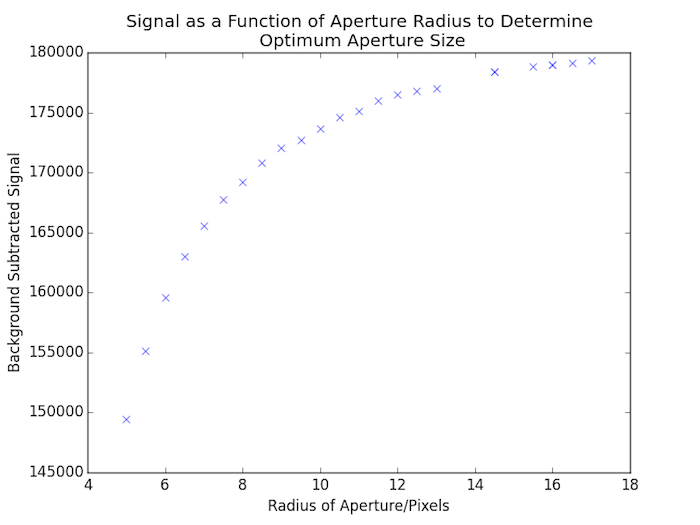
\includegraphics[scale = 0.4]{/Users/tomasjames/Documents/University/Cardiff/Project/Project/Reports/Interim/Master/img/aperture_qatar1b.png}
\caption[An example of how the optimum aperture size was determined by observing how the background subtracted signal varies with aperture size. The point at which the gradient of the curve becomes constant - in this instance at the 12 pixel point - is the optimum aperture size.]{An example of how the optimum aperture size was determined by observing how the background subtracted signal varies with aperture size. The point at which the gradient of the curve becomes constant - in this instance at the 12 pixel point - is the optimum aperture size.} \label{qatar1b}
\end{figure}

As the aperture size increases, so does the measured count inside of the aperture. When all of the star's flux has been measured, any further increase in aperture size will detect a uniform, constant background leading to a constant increase in the count. This is manifested graphically by a constant gradient. The point at which the graph plateaus is the optimum aperture size.

For a transit ingress to be reliably observed differential aperture photometry is performed in addition to the above using equation \ref{diffphotom}. 

\begin{equation} \label{diffphotom}
    S = \frac{F_{i}}{F_{c}-F_{b}}
\end{equation}

In equation \ref{diffphotom}, $S$ is the calibrated flux, $F_{i}$ is the incident flux as defined earlier, $F_{c}$ is the calibration star flux and $F_{b}$ is the background flux.

This essentially calibrates the flux from the object of interest against another object of similar brightness in the field of view. Providing that the calibration star has constant luminosity (and therefore constant flux) this `normalises' the count. For reliability and comparison this is performed with as many different calibration stars as the field of view allows.

This procedure is repeated across an even number of exposures, evenly distributed across the transit and, importantly, about its transit centre. A Python script was then written to plot $S$ as a function of time, thereby producing a light curve.

%-----------------------------------------------------------------
% Future Work
%-----------------------------------------------------------------

\section{Future Work}
Future work will focus on analysing the data collected for each observed transit. Differential aperture photometry will be performed on the data, and a physical model will be fitted to the resulting light curves to better characterise the exoplanets.Properties such as mass and orbital period will then be calculated from this analysed data and compared and contrasted between each other, as well as to the known values. The modelling procedure outlined by \textcite{model} will be used in order to accomplish this. [Is this last part particularly relevant?]

%-----------------------------------------------------------------
% Bibliography
%-----------------------------------------------------------------

\nocite{*}
\printbibliography

\label{lastpage}

\end{document}
